\documentclass[11pt]{article}
% ============================================================================
% Single-file manuscript. Preamble and palette are inlined below rather than
% \input from separate files, deliberately.
%
% figs/rna_numbers.tex is the ONE include, and it is generated: make_numbers.py
% writes every \jdg{} macro from the committed run artifacts in
% rna_harness/runs/ceiling/. It is data, not a chapter. No measured number is
% typed into this file by hand, so a printed figure cannot drift from its run.
%
% Build:  python make_figs.py && python make_numbers.py && tectonic -X compile R1_placement.tex
% ============================================================================

% ------------------------------------------------ preamble
% Shared preamble. Layout and environments follow the T6 judge manuscript so the two read as one
% family; nothing here is specific to this paper's content.
\usepackage[margin=1in]{geometry}
\usepackage[utf8]{inputenc}
\usepackage[T1]{fontenc}
\usepackage{textcomp}
\usepackage{amsmath,amssymb,amsthm,amsfonts}
\usepackage{booktabs}
\usepackage{graphicx}
\usepackage{xcolor}
\usepackage{array}
\usepackage{enumitem}
\usepackage{placeins}
\usepackage{tabularx}
\usepackage[hidelinks]{hyperref}
\usepackage[numbers,sort&compress]{natbib}
\usepackage{authblk}
\usepackage{caption}
\usepackage{tcolorbox}
\tcbuselibrary{skins,breakable}
\captionsetup{font=small,labelfont=bf,skip=4pt}
\emergencystretch=1.5em
\graphicspath{{figs/}}

\renewcommand{\topfraction}{0.92}
\renewcommand{\bottomfraction}{0.85}
\renewcommand{\textfraction}{0.06}
\renewcommand{\floatpagefraction}{0.72}
\setcounter{topnumber}{4}\setcounter{bottomnumber}{3}\setcounter{totalnumber}{6}

\newtheorem{proposition}{Proposition}
\newtheorem{definition}{Definition}
\newtheorem{assumption}{Assumption}

% ---------------------------------------------------------------- generated numbers
% \jdg{name} prints a number defined in figs/rna_numbers.tex, which make_numbers.py writes from
% the committed run artifacts. An undefined name is a build error rather than a silent blank,
% because a missing measurement must not print as nothing.
\newcommand{\jdg}[1]{%
  \ifcsname jdg@#1\endcsname\csname jdg@#1\endcsname
  \else\textbf{??#1??}\PackageError{rna}{undefined measured quantity #1}{}\fi}

% ---------------------------------------------------------------- boxes
\newtcolorbox{claimbox}{breakable,enhanced,colback=cbBack,colframe=cbLine,
  boxrule=0.6pt,left=6pt,right=6pt,top=5pt,bottom=5pt,arc=1pt}
\newtcolorbox{scopebox}{breakable,enhanced,colback=sbBack,colframe=sbLine,
  boxrule=0.6pt,left=6pt,right=6pt,top=5pt,bottom=5pt,arc=1pt,
  borderline west={2pt}{0pt}{sbLine}}

% ------------------------------------------------ palette
% Palette. Series colours are the three dataviz reference slots used by every figure in this
% family; the ink tokens are text only and are never used for a data series.
\definecolor{S1}{HTML}{2A78D6}
\definecolor{S2}{HTML}{EB6834}
\definecolor{S3}{HTML}{1BAF7A}
\definecolor{INK}{HTML}{0B0B0B}
\definecolor{INKB}{HTML}{52514E}
\definecolor{INKC}{HTML}{8A8984}
\definecolor{cbBack}{HTML}{F4F8FD}
\definecolor{cbLine}{HTML}{2A78D6}
\definecolor{sbBack}{HTML}{FBF6F2}
\definecolor{sbLine}{HTML}{EB6834}

% ------------------------------------------------ generated numbers (the only include)
% GENERATED by make_numbers.py from rna_harness/runs/ceiling/*.json.
% Do not edit. Do not type a measured number into the manuscript by hand.
\expandafter\def\csname jdg@a7BinderRatio\endcsname{10.29}
\expandafter\def\csname jdg@a7Bins\endcsname{+0.1087, +0.1067}
\expandafter\def\csname jdg@a7Failed\endcsname{$P_{\mathrm{model}}$ and binder length}
\expandafter\def\csname jdg@a7Held\endcsname{$\Delta G_{\mathrm{loc}}$ and helix depth}
\expandafter\def\csname jdg@a7Mean\endcsname{+0.1077}
\expandafter\def\csname jdg@a7N\endcsname{2}
\expandafter\def\csname jdg@a7NAll\endcsname{4}
\expandafter\def\csname jdg@a7NHeld\endcsname{2}
\expandafter\def\csname jdg@a7PmutRatio\endcsname{2.94}
\expandafter\def\csname jdg@a7Ratio\endcsname{0.018}
\expandafter\def\csname jdg@a7Spread\endcsname{0.0019}
\expandafter\def\csname jdg@c5Cut\endcsname{0.80}
\expandafter\def\csname jdg@c5N\endcsname{6}
\expandafter\def\csname jdg@c5Sig\endcsname{4}
\expandafter\def\csname jdg@cEffHi\endcsname{+3.79}
\expandafter\def\csname jdg@cEffLo\endcsname{+2.12}
\expandafter\def\csname jdg@cSigLoose\endcsname{6}
\expandafter\def\csname jdg@cSigStrict\endcsname{4}
\expandafter\def\csname jdg@cSmdHi\endcsname{0.039}
\expandafter\def\csname jdg@cZHi\endcsname{7.7}
\expandafter\def\csname jdg@cZLo\endcsname{1.7}
\expandafter\def\csname jdg@calNAlpha\endcsname{+0.06055}
\expandafter\def\csname jdg@calNBound\endcsname{23.2\%}
\expandafter\def\csname jdg@calNCorr\endcsname{-0.7019}
\expandafter\def\csname jdg@calNFull\endcsname{+131.4\%}
\expandafter\def\csname jdg@calNLoo\endcsname{-0.0628}
\expandafter\def\csname jdg@calNLooHi\endcsname{-0.0628}
\expandafter\def\csname jdg@calNLooLo\endcsname{-0.8400}
\expandafter\def\csname jdg@calNMae\endcsname{0.4743}
\expandafter\def\csname jdg@calNRho\endcsname{-0.3143}
\expandafter\def\csname jdg@calNSpan\endcsname{0.0967}
\expandafter\def\csname jdg@calNSpanFrac\endcsname{12.9\%}
\expandafter\def\csname jdg@calNThr\endcsname{500}
\expandafter\def\csname jdg@calNZero\endcsname{103.2\%}
\expandafter\def\csname jdg@calOutSd\endcsname{0.2501}
\expandafter\def\csname jdg@calSpanTop\endcsname{75\%}
\expandafter\def\csname jdg@calSpanTrue\endcsname{0.75}
\expandafter\def\csname jdg@calStdC\endcsname{0.216}
\expandafter\def\csname jdg@calStdCThr\endcsname{0.2}
\expandafter\def\csname jdg@calSweep\endcsname{0\%, 10\%, 25\%, 50\%, 75\%, 100\%}
\expandafter\def\csname jdg@calTotal\endcsname{+0.05393}
\expandafter\def\csname jdg@calVAlpha\endcsname{-0.03039}
\expandafter\def\csname jdg@calVBound\endcsname{6.8\%}
\expandafter\def\csname jdg@calVCorr\endcsname{+0.7026}
\expandafter\def\csname jdg@calVFull\endcsname{-842.5\%}
\expandafter\def\csname jdg@calVLoo\endcsname{-0.7613}
\expandafter\def\csname jdg@calVLooHi\endcsname{+0.8794}
\expandafter\def\csname jdg@calVLooLo\endcsname{-0.7613}
\expandafter\def\csname jdg@calVMae\endcsname{1.7358}
\expandafter\def\csname jdg@calVRho\endcsname{+0.0286}
\expandafter\def\csname jdg@calVSpan\endcsname{0.2154}
\expandafter\def\csname jdg@calVSpanFrac\endcsname{28.7\%}
\expandafter\def\csname jdg@calVZero\endcsname{95.7\%}
\expandafter\def\csname jdg@cbAtBins\endcsname{13}
\expandafter\def\csname jdg@cbBinHi\endcsname{23}
\expandafter\def\csname jdg@cbBinLo\endcsname{3}
\expandafter\def\csname jdg@cbCiBoot\endcsname{400}
\expandafter\def\csname jdg@cbCiHi\endcsname{135.8\%}
\expandafter\def\csname jdg@cbCiLo\endcsname{37.8\%}
\expandafter\def\csname jdg@cbCiMed\endcsname{57.9\%}
\expandafter\def\csname jdg@cbCiVac\endcsname{7.8\%}
\expandafter\def\csname jdg@cbDtvHi\endcsname{0.750}
\expandafter\def\csname jdg@cbDtvLo\endcsname{0.417}
\expandafter\def\csname jdg@cbLoose\endcsname{101.9\%}
\expandafter\def\csname jdg@cbNbins\endcsname{8}
\expandafter\def\csname jdg@cbOscHi\endcsname{0.1154}
\expandafter\def\csname jdg@cbOscLo\endcsname{0.0309}
\expandafter\def\csname jdg@cbPmTight\endcsname{11.5\%}
\expandafter\def\csname jdg@cbRhoLhs\endcsname{+0.262}
\expandafter\def\csname jdg@cbRhoRhs\endcsname{+1.000}
\expandafter\def\csname jdg@cbTight\endcsname{53.1\%}
\expandafter\def\csname jdg@cbTightHi\endcsname{60.6\%}
\expandafter\def\csname jdg@cbTightLo\endcsname{53.1\%}
\expandafter\def\csname jdg@ccCellsR\endcsname{158}
\expandafter\def\csname jdg@ccPuzzlesR\endcsname{20}
\expandafter\def\csname jdg@ceilA\endcsname{0.8793}
\expandafter\def\csname jdg@ceilACi\endcsname{[0.8469,\,0.9107]}
\expandafter\def\csname jdg@ceilB\endcsname{0.6956}
\expandafter\def\csname jdg@ceilBCi\endcsname{[0.6422,\,0.7441]}
\expandafter\def\csname jdg@ceilDeclared\endcsname{2.897}
\expandafter\def\csname jdg@ceilDf\endcsname{1426}
\expandafter\def\csname jdg@ceilGroups\endcsname{557}
\expandafter\def\csname jdg@ceilHeavyTail\endcsname{1.35}
\expandafter\def\csname jdg@ceilNormalTail\endcsname{1.18}
\expandafter\def\csname jdg@ceilPairs\endcsname{454}
\expandafter\def\csname jdg@ceilRms454\endcsname{4.3469}
\expandafter\def\csname jdg@ceilRows\endcsname{1983}
\expandafter\def\csname jdg@ceilSigA\endcsname{2.3755}
\expandafter\def\csname jdg@ceilSigACi\endcsname{[2.0428,\,2.6749]}
\expandafter\def\csname jdg@ceilSigB\endcsname{3.7716}
\expandafter\def\csname jdg@ceilSigBCi\endcsname{[3.4585,\,4.0891]}
\expandafter\def\csname jdg@ceilWithinSd\endcsname{6.8362}
\expandafter\def\csname jdg@cpop0Ci\endcsname{[2.43,\,4.96]}
\expandafter\def\csname jdg@cpop0Eff\endcsname{+3.682}
\expandafter\def\csname jdg@cpop0N\endcsname{3308}
\expandafter\def\csname jdg@cpop0P\endcsname{0.0005}
\expandafter\def\csname jdg@cpop0Smd\endcsname{0.039}
\expandafter\def\csname jdg@cpop0SmdP\endcsname{0.002}
\expandafter\def\csname jdg@cpop0Z\endcsname{7.72}
\expandafter\def\csname jdg@cpop1Ci\endcsname{[2.36,\,5.44]}
\expandafter\def\csname jdg@cpop1Eff\endcsname{+3.794}
\expandafter\def\csname jdg@cpop1N\endcsname{700}
\expandafter\def\csname jdg@cpop1P\endcsname{0.0005}
\expandafter\def\csname jdg@cpop1Smd\endcsname{0.031}
\expandafter\def\csname jdg@cpop1SmdP\endcsname{0.004}
\expandafter\def\csname jdg@cpop1Z\endcsname{5.60}
\expandafter\def\csname jdg@cpop2Ci\endcsname{[1.33,\,5.18]}
\expandafter\def\csname jdg@cpop2Eff\endcsname{+3.232}
\expandafter\def\csname jdg@cpop2N\endcsname{634}
\expandafter\def\csname jdg@cpop2P\endcsname{0.0005}
\expandafter\def\csname jdg@cpop2Smd\endcsname{0.038}
\expandafter\def\csname jdg@cpop2SmdP\endcsname{0.000}
\expandafter\def\csname jdg@cpop2Z\endcsname{4.12}
\expandafter\def\csname jdg@cpop3Ci\endcsname{[0.04,\,4.29]}
\expandafter\def\csname jdg@cpop3Eff\endcsname{+2.122}
\expandafter\def\csname jdg@cpop3N\endcsname{222}
\expandafter\def\csname jdg@cpop3P\endcsname{0.0165}
\expandafter\def\csname jdg@cpop3Smd\endcsname{0.038}
\expandafter\def\csname jdg@cpop3SmdP\endcsname{0.004}
\expandafter\def\csname jdg@cpop3Z\endcsname{2.08}
\expandafter\def\csname jdg@cpop4Ci\endcsname{[1.10,\,6.29]}
\expandafter\def\csname jdg@cpop4Eff\endcsname{+3.708}
\expandafter\def\csname jdg@cpop4N\endcsname{174}
\expandafter\def\csname jdg@cpop4P\endcsname{0.0020}
\expandafter\def\csname jdg@cpop4Smd\endcsname{0.034}
\expandafter\def\csname jdg@cpop4SmdP\endcsname{0.007}
\expandafter\def\csname jdg@cpop4Z\endcsname{3.14}
\expandafter\def\csname jdg@cpop5Ci\endcsname{[-0.24,\,6.58]}
\expandafter\def\csname jdg@cpop5Eff\endcsname{+3.522}
\expandafter\def\csname jdg@cpop5N\endcsname{45}
\expandafter\def\csname jdg@cpop5P\endcsname{0.0450}
\expandafter\def\csname jdg@cpop5Smd\endcsname{0.033}
\expandafter\def\csname jdg@cpop5SmdP\endcsname{0.001}
\expandafter\def\csname jdg@cpop5Z\endcsname{1.70}
\expandafter\def\csname jdg@cxBase\endcsname{+0.0407}
\expandafter\def\csname jdg@cxCi0\endcsname{[$+0.0012$, $+0.0525$]}
\expandafter\def\csname jdg@cxCi1\endcsname{[$-0.0014$, $+0.0514$]}
\expandafter\def\csname jdg@cxCi2\endcsname{[$-0.0036$, $+0.0477$]}
\expandafter\def\csname jdg@cxCi3\endcsname{[$-0.0094$, $+0.0451$]}
\expandafter\def\csname jdg@cxE0\endcsname{+0.0274}
\expandafter\def\csname jdg@cxE1\endcsname{+0.0260}
\expandafter\def\csname jdg@cxE2\endcsname{+0.0229}
\expandafter\def\csname jdg@cxE3\endcsname{+0.0194}
\expandafter\def\csname jdg@cxOnlyE\endcsname{+0.0481}
\expandafter\def\csname jdg@cxOnlyN\endcsname{4235}
\expandafter\def\csname jdg@cxOnlyShare\endcsname{118\%}
\expandafter\def\csname jdg@cxP0\endcsname{0.0015}
\expandafter\def\csname jdg@cxP1\endcsname{0.0030}
\expandafter\def\csname jdg@cxP2\endcsname{0.0105}
\expandafter\def\csname jdg@cxP3\endcsname{0.0305}
\expandafter\def\csname jdg@cxReleased\endcsname{+0.0539}
\expandafter\def\csname jdg@cxRet0\endcsname{67\%}
\expandafter\def\csname jdg@cxRet1\endcsname{64\%}
\expandafter\def\csname jdg@cxRet2\endcsname{56\%}
\expandafter\def\csname jdg@cxRet3\endcsname{48\%}
\expandafter\def\csname jdg@cxSites0\endcsname{98}
\expandafter\def\csname jdg@cxSites1\endcsname{94}
\expandafter\def\csname jdg@cxSites2\endcsname{90}
\expandafter\def\csname jdg@cxSites3\endcsname{86}
\expandafter\def\csname jdg@d2C04\endcsname{0}
\expandafter\def\csname jdg@d2C06\endcsname{1}
\expandafter\def\csname jdg@d2C08\endcsname{0}
\expandafter\def\csname jdg@d2C10\endcsname{0}
\expandafter\def\csname jdg@d2CHi\endcsname{1}
\expandafter\def\csname jdg@d2CLo\endcsname{0}
\expandafter\def\csname jdg@d2P04\endcsname{5}
\expandafter\def\csname jdg@d2P06\endcsname{5}
\expandafter\def\csname jdg@d2P08\endcsname{3}
\expandafter\def\csname jdg@d2P10\endcsname{2}
\expandafter\def\csname jdg@d2PHi\endcsname{5}
\expandafter\def\csname jdg@d2PLo\endcsname{2}
\expandafter\def\csname jdg@d2SlopeC04\endcsname{10.3}
\expandafter\def\csname jdg@d2SlopeC06\endcsname{10.6}
\expandafter\def\csname jdg@d2SlopeC08\endcsname{-1.7}
\expandafter\def\csname jdg@d2SlopeC10\endcsname{20.0}
\expandafter\def\csname jdg@d2SlopeP04\endcsname{54.5}
\expandafter\def\csname jdg@d2SlopeP06\endcsname{53.4}
\expandafter\def\csname jdg@d2SlopeP08\endcsname{37.9}
\expandafter\def\csname jdg@d2SlopeP10\endcsname{41.2}
\expandafter\def\csname jdg@d3E0\endcsname{-4.411}
\expandafter\def\csname jdg@d3E0Ci\endcsname{[-5.38,\,-3.48]}
\expandafter\def\csname jdg@d3E1\endcsname{-5.160}
\expandafter\def\csname jdg@d3E1Ci\endcsname{[-6.17,\,-4.27]}
\expandafter\def\csname jdg@d3E2\endcsname{-3.740}
\expandafter\def\csname jdg@d3E2Ci\endcsname{[-4.63,\,-2.94]}
\expandafter\def\csname jdg@d3E3\endcsname{-4.951}
\expandafter\def\csname jdg@d3E3Ci\endcsname{[-5.87,\,-4.14]}
\expandafter\def\csname jdg@d3NNeg\endcsname{4}
\expandafter\def\csname jdg@d3NPos\endcsname{4}
\expandafter\def\csname jdg@d3Y0\endcsname{+0.1982}
\expandafter\def\csname jdg@d3Y0Ci\endcsname{[0.172,\,0.221]}
\expandafter\def\csname jdg@d3Y1\endcsname{+0.5049}
\expandafter\def\csname jdg@d3Y1Ci\endcsname{[0.443,\,0.569]}
\expandafter\def\csname jdg@d3Y2\endcsname{+0.3187}
\expandafter\def\csname jdg@d3Y2Ci\endcsname{[0.276,\,0.366]}
\expandafter\def\csname jdg@d3Y3\endcsname{+0.4282}
\expandafter\def\csname jdg@d3Y3Ci\endcsname{[0.382,\,0.477]}
\expandafter\def\csname jdg@dBoundRatio\endcsname{8.6}
\expandafter\def\csname jdg@dDg\endcsname{-1.7245}
\expandafter\def\csname jdg@dDgBound\endcsname{58.6\%}
\expandafter\def\csname jdg@dDgCi\endcsname{[-1.8088,\,\allowbreak -1.6333]}
\expandafter\def\csname jdg@dDgP\endcsname{<0.001}
\expandafter\def\csname jdg@dDgSlope\endcsname{-0.01833}
\expandafter\def\csname jdg@dN\endcsname{4317}
\expandafter\def\csname jdg@dOut\endcsname{+0.0539}
\expandafter\def\csname jdg@dOutCi\endcsname{[+0.0220,\,\allowbreak +0.0956]}
\expandafter\def\csname jdg@dOutP\endcsname{<0.001}
\expandafter\def\csname jdg@dPm\endcsname{-0.0304}
\expandafter\def\csname jdg@dPmBound\endcsname{6.8\%}
\expandafter\def\csname jdg@dPmCi\endcsname{[-0.0637,\,\allowbreak +0.0042]}
\expandafter\def\csname jdg@dPmP\endcsname{0.0545}
\expandafter\def\csname jdg@dPmSlope\endcsname{+0.12059}
\expandafter\def\csname jdg@dStrata\endcsname{553}
\expandafter\def\csname jdg@dW\endcsname{902}
\expandafter\def\csname jdg@dgBase\endcsname{+3.682}
\expandafter\def\csname jdg@dgLooseCal\endcsname{7.05}
\expandafter\def\csname jdg@dgLooseEff\endcsname{+3.862}
\expandafter\def\csname jdg@dgLooseP\endcsname{0.0010}
\expandafter\def\csname jdg@dgRetain\endcsname{81\%}
\expandafter\def\csname jdg@dgSd\endcsname{7.05}
\expandafter\def\csname jdg@dgTightCal\endcsname{0.44}
\expandafter\def\csname jdg@dgTightEff\endcsname{+2.991}
\expandafter\def\csname jdg@dgTightP\endcsname{0.0200}
\expandafter\def\csname jdg@dgmAu\endcsname{0.2877}
\expandafter\def\csname jdg@dgmCg\endcsname{0.3211}
\expandafter\def\csname jdg@dgmGu\endcsname{0.3047}
\expandafter\def\csname jdg@dgmNAu\endcsname{2232}
\expandafter\def\csname jdg@dgmNCg\endcsname{6122}
\expandafter\def\csname jdg@dgmNGu\endcsname{280}
\expandafter\def\csname jdg@dgmOldAu\endcsname{0.2881}
\expandafter\def\csname jdg@dgmOldCg\endcsname{0.3261}
\expandafter\def\csname jdg@dgmOldGu\endcsname{0.3076}
\expandafter\def\csname jdg@dnD\endcsname{+0.0700}
\expandafter\def\csname jdg@dnDCi\endcsname{[$+0.0560$, $+0.0828$]}
\expandafter\def\csname jdg@dnDenShare\endcsname{61\%}
\expandafter\def\csname jdg@dnFromDen\endcsname{+0.0939}
\expandafter\def\csname jdg@dnFromNum\endcsname{\ensuremath{-}0.0591}
\expandafter\def\csname jdg@dnNum\endcsname{+0.0262}
\expandafter\def\csname jdg@dnNumCi\endcsname{[$+0.0115$, $+0.0439$]}
\expandafter\def\csname jdg@doseEff0\endcsname{+2.754}
\expandafter\def\csname jdg@doseEff1\endcsname{+6.214}
\expandafter\def\csname jdg@doseEff2\endcsname{+6.744}
\expandafter\def\csname jdg@doseLo0\endcsname{0.05}
\expandafter\def\csname jdg@doseLo1\endcsname{0.10}
\expandafter\def\csname jdg@doseLo2\endcsname{0.15}
\expandafter\def\csname jdg@doseN0\endcsname{2460}
\expandafter\def\csname jdg@doseN1\endcsname{594}
\expandafter\def\csname jdg@doseN2\endcsname{254}
\expandafter\def\csname jdg@eBaseFull\endcsname{+0.0539}
\expandafter\def\csname jdg@eBaseSame\endcsname{+0.0805}
\expandafter\def\csname jdg@eBeta\endcsname{-0.02286}
\expandafter\def\csname jdg@eBinsAU\endcsname{0/73/436/258/349}
\expandafter\def\csname jdg@eBinsCG\endcsname{776/871/392/584/438}
\expandafter\def\csname jdg@eBinsGU\endcsname{0/0/33/20/87}
\expandafter\def\csname jdg@eBinwise\endcsname{-0.0085,\;+0.0214,\;+0.0122,\;-0.0019,\;-0.0222}
\expandafter\def\csname jdg@eBinwiseDg\endcsname{-6.45,\;-5.34,\;-3.94,\;-3.18,\;-1.46}
\expandafter\def\csname jdg@eCde\endcsname{+0.0820}
\expandafter\def\csname jdg@eCi\endcsname{[0.0488,\,0.1201]}
\expandafter\def\csname jdg@eContam\endcsname{233}
\expandafter\def\csname jdg@eContamPct\endcsname{5.2\%}
\expandafter\def\csname jdg@eDOne\endcsname{+0.0124}
\expandafter\def\csname jdg@eDOneN\endcsname{1378}
\expandafter\def\csname jdg@eDOneP\endcsname{0.2229}
\expandafter\def\csname jdg@eDOneW\endcsname{288}
\expandafter\def\csname jdg@eDTwo\endcsname{+0.0608}
\expandafter\def\csname jdg@eDTwoN\endcsname{1522}
\expandafter\def\csname jdg@eDTwoP\endcsname{0.0005}
\expandafter\def\csname jdg@eDTwoW\endcsname{394}
\expandafter\def\csname jdg@eDZero\endcsname{+0.0922}
\expandafter\def\csname jdg@eDZeroN\endcsname{1553}
\expandafter\def\csname jdg@eDZeroP\endcsname{0.0005}
\expandafter\def\csname jdg@eDZeroW\endcsname{246}
\expandafter\def\csname jdg@eDeltaZero\endcsname{0.00}
\expandafter\def\csname jdg@eDgAU\endcsname{-3.002}
\expandafter\def\csname jdg@eDgCG\endcsname{-4.592}
\expandafter\def\csname jdg@eDgGU\endcsname{-1.859}
\expandafter\def\csname jdg@eDgSdAU\endcsname{1.309}
\expandafter\def\csname jdg@eDgSdCG\endcsname{1.578}
\expandafter\def\csname jdg@eDgSdGU\endcsname{1.552}
\expandafter\def\csname jdg@eDgdag\endcsname{-0.5041}
\expandafter\def\csname jdg@eDgdca\endcsname{-1.7245}
\expandafter\def\csname jdg@eDgdcg\endcsname{-2.3814}
\expandafter\def\csname jdg@eGap\endcsname{-1.7245}
\expandafter\def\csname jdg@eGuAdj\endcsname{+0.1711}
\expandafter\def\csname jdg@eGuAdjN\endcsname{31}
\expandafter\def\csname jdg@eGuIso\endcsname{+0.0893}
\expandafter\def\csname jdg@eGuIsoN\endcsname{109}
\expandafter\def\csname jdg@eLad\endcsname{0.10}
\expandafter\def\csname jdg@eLinearGapPts\endcsname{75.0}
\expandafter\def\csname jdg@eLinearMed\endcsname{73.1\%}
\expandafter\def\csname jdg@eMaxDgChange\endcsname{3.00}
\expandafter\def\csname jdg@eMed\endcsname{-1.9\%}
\expandafter\def\csname jdg@eMedCi\endcsname{[-10.6\%,\,+6.8\%]}
\expandafter\def\csname jdg@eNBins\endcsname{5}
\expandafter\def\csname jdg@eNoise\endcsname{0}
\expandafter\def\csname jdg@eNullSd\endcsname{0.0158}
\expandafter\def\csname jdg@eP\endcsname{0.0005}
\expandafter\def\csname jdg@ePlaceboHi\endcsname{107.0\%}
\expandafter\def\csname jdg@ePlaceboLo\endcsname{93.2\%}
\expandafter\def\csname jdg@ePlaceboMean\endcsname{100.9\%}
\expandafter\def\csname jdg@ePlaceboSd\endcsname{4.4}
\expandafter\def\csname jdg@eProbe\endcsname{+1.30}
\expandafter\def\csname jdg@eRet\endcsname{101.9\%}
\expandafter\def\csname jdg@eRetWrong\endcsname{152.1\%}
\expandafter\def\csname jdg@eSel\endcsname{149.3\%}
\expandafter\def\csname jdg@eSens3\endcsname{100.1\%}
\expandafter\def\csname jdg@eSens8\endcsname{100.9\%}
\expandafter\def\csname jdg@eSlopeSpread\endcsname{1.77}
\expandafter\def\csname jdg@eSlopeag\endcsname{-0.05533}
\expandafter\def\csname jdg@eSlopeca\endcsname{-0.03127}
\expandafter\def\csname jdg@eSlopecg\endcsname{-0.04389}
\expandafter\def\csname jdg@eStrata\endcsname{285}
\expandafter\def\csname jdg@eTermAU\endcsname{0.50}
\expandafter\def\csname jdg@eW\endcsname{363}
\expandafter\def\csname jdg@eWBase\endcsname{367}
\expandafter\def\csname jdg@eZ\endcsname{+0.22}
\expandafter\def\csname jdg@gCells\endcsname{117}
\expandafter\def\csname jdg@gGapMax\endcsname{-0.7118}
\expandafter\def\csname jdg@gGapMaxName\endcsname{Eterna}
\expandafter\def\csname jdg@gGapMin\endcsname{-0.1271}
\expandafter\def\csname jdg@gGapMinName\endcsname{MPNN-RFdiff}
\expandafter\def\csname jdg@gHumanRank\endcsname{0}
\expandafter\def\csname jdg@gLadHi\endcsname{0.92}
\expandafter\def\csname jdg@gLadLo\endcsname{0.08}
\expandafter\def\csname jdg@gLadZero\endcsname{0.00}
\expandafter\def\csname jdg@gMethComp\endcsname{0.1200}
\expandafter\def\csname jdg@gNMethods\endcsname{9}
\expandafter\def\csname jdg@gNoise\endcsname{0}
\expandafter\def\csname jdg@gNullMean\endcsname{0.0525}
\expandafter\def\csname jdg@gNullSd\endcsname{0.0243}
\expandafter\def\csname jdg@gP\endcsname{0.0120}
\expandafter\def\csname jdg@gRatio\endcsname{5.6}
\expandafter\def\csname jdg@gSlope\endcsname{0.836}
\expandafter\def\csname jdg@gSlopeN\endcsname{9}
\expandafter\def\csname jdg@gSlopeP\endcsname{0.0070}
\expandafter\def\csname jdg@gSpread\endcsname{0.585}
\expandafter\def\csname jdg@gTgtComp\endcsname{0.6477}
\expandafter\def\csname jdg@gZ\endcsname{2.78}
\expandafter\def\csname jdg@imbBetaHi\endcsname{28.7}
\expandafter\def\csname jdg@imbBetaLo\endcsname{16.1}
\expandafter\def\csname jdg@imbDpiFreeHi\endcsname{2.76}
\expandafter\def\csname jdg@imbDpiFreeLo\endcsname{1.50}
\expandafter\def\csname jdg@imbDpiPanHi\endcsname{0.014}
\expandafter\def\csname jdg@imbDpiPanLo\endcsname{-0.024}
\expandafter\def\csname jdg@imbFreeHi\endcsname{37.7\%}
\expandafter\def\csname jdg@imbFreeLo\endcsname{22.8\%}
\expandafter\def\csname jdg@imbPanHi\endcsname{3.16\%}
\expandafter\def\csname jdg@imbPanLo\endcsname{0.95\%}
\expandafter\def\csname jdg@lbBMaxMove\endcsname{3}
\expandafter\def\csname jdg@lbBMoved\endcsname{7}
\expandafter\def\csname jdg@lbBMovedTarget\endcsname{0}
\expandafter\def\csname jdg@lbBN\endcsname{22879}
\expandafter\def\csname jdg@lbBNMeth\endcsname{12}
\expandafter\def\csname jdg@lbBNewTop\endcsname{Struct2SeQ}
\expandafter\def\csname jdg@lbBNewTopOld\endcsname{3}
\expandafter\def\csname jdg@lbBTau\endcsname{+0.697}
\expandafter\def\csname jdg@lbBTauCi\endcsname{[$+0.636$, $+0.849$]}
\expandafter\def\csname jdg@lbBTauTarget\endcsname{+1.000}
\expandafter\def\csname jdg@lbBTop\endcsname{codesign-RFdiff}
\expandafter\def\csname jdg@lbBTopNew\endcsname{4}
\expandafter\def\csname jdg@lbMaxMove\endcsname{1}
\expandafter\def\csname jdg@lbMoved\endcsname{2}
\expandafter\def\csname jdg@lbMovedTarget\endcsname{4}
\expandafter\def\csname jdg@lbNMeth\endcsname{9}
\expandafter\def\csname jdg@lbStrata\endcsname{915}
\expandafter\def\csname jdg@lbTau\endcsname{+0.944}
\expandafter\def\csname jdg@lbTauCi\endcsname{[$+0.778$, $+1.000$]}
\expandafter\def\csname jdg@lbTauTarget\endcsname{+0.889}
\expandafter\def\csname jdg@legN\endcsname{152}
\expandafter\def\csname jdg@legRho\endcsname{+0.228}
\expandafter\def\csname jdg@legRhoP\endcsname{0.006}
\expandafter\def\csname jdg@legSdRatio\endcsname{2.04}
\expandafter\def\csname jdg@legSlope\endcsname{+0.04943}
\expandafter\def\csname jdg@legSlopeP\endcsname{0.1894}
\expandafter\def\csname jdg@m15pop0Comp\endcsname{56}
\expandafter\def\csname jdg@m15pop0Eff\endcsname{+3.727}
\expandafter\def\csname jdg@m15pop0N\endcsname{2030}
\expandafter\def\csname jdg@m15pop0P\endcsname{0.0005}
\expandafter\def\csname jdg@m15pop0Pass\endcsname{6839}
\expandafter\def\csname jdg@m15pop0Ref\endcsname{+3.682}
\expandafter\def\csname jdg@m15pop1Comp\endcsname{13}
\expandafter\def\csname jdg@m15pop1Eff\endcsname{+4.278}
\expandafter\def\csname jdg@m15pop1N\endcsname{422}
\expandafter\def\csname jdg@m15pop1P\endcsname{0.0005}
\expandafter\def\csname jdg@m15pop1Pass\endcsname{3371}
\expandafter\def\csname jdg@m15pop1Ref\endcsname{+3.794}
\expandafter\def\csname jdg@m15pop2Comp\endcsname{10}
\expandafter\def\csname jdg@m15pop2Eff\endcsname{+2.744}
\expandafter\def\csname jdg@m15pop2N\endcsname{477}
\expandafter\def\csname jdg@m15pop2P\endcsname{0.0005}
\expandafter\def\csname jdg@m15pop2Pass\endcsname{3414}
\expandafter\def\csname jdg@m15pop2Ref\endcsname{+3.232}
\expandafter\def\csname jdg@m15pop3Comp\endcsname{13}
\expandafter\def\csname jdg@m15pop3Eff\endcsname{+1.990}
\expandafter\def\csname jdg@m15pop3N\endcsname{116}
\expandafter\def\csname jdg@m15pop3P\endcsname{0.0265}
\expandafter\def\csname jdg@m15pop3Pass\endcsname{1854}
\expandafter\def\csname jdg@m15pop3Ref\endcsname{+2.122}
\expandafter\def\csname jdg@m15pop4Comp\endcsname{1}
\expandafter\def\csname jdg@m15pop4Eff\endcsname{+3.945}
\expandafter\def\csname jdg@m15pop4N\endcsname{132}
\expandafter\def\csname jdg@m15pop4P\endcsname{0.0005}
\expandafter\def\csname jdg@m15pop4Pass\endcsname{1007}
\expandafter\def\csname jdg@m15pop4Ref\endcsname{+3.708}
\expandafter\def\csname jdg@m15pop5Comp\endcsname{9}
\expandafter\def\csname jdg@m15pop5Eff\endcsname{+4.869}
\expandafter\def\csname jdg@m15pop5N\endcsname{16}
\expandafter\def\csname jdg@m15pop5P\endcsname{0.0535}
\expandafter\def\csname jdg@m15pop5Pass\endcsname{809}
\expandafter\def\csname jdg@m15pop5Ref\endcsname{+3.522}
\expandafter\def\csname jdg@m23BlockMed\endcsname{1.0}
\expandafter\def\csname jdg@m23CrossBlock\endcsname{44.4\%}
\expandafter\def\csname jdg@m23Dgp3Leak\endcsname{47.5\%}
\expandafter\def\csname jdg@m23LeakCorr\endcsname{+0.857}
\expandafter\def\csname jdg@m23LeakHi\endcsname{33.7\%}
\expandafter\def\csname jdg@m23LeakLo\endcsname{4.7\%}
\expandafter\def\csname jdg@m23Ratio\endcsname{8.9}
\expandafter\def\csname jdg@m23nBl\endcsname{0.000}
\expandafter\def\csname jdg@m23nBlN\endcsname{0/240}
\expandafter\def\csname jdg@m23nFL\endcsname{0.000}
\expandafter\def\csname jdg@m23nFLN\endcsname{0/240}
\expandafter\def\csname jdg@m23nT\endcsname{0.037}
\expandafter\def\csname jdg@m23nTN\endcsname{9/240}
\expandafter\def\csname jdg@m23nY\endcsname{0.004}
\expandafter\def\csname jdg@m23nYN\endcsname{1/240}
\expandafter\def\csname jdg@medBeta\endcsname{0.0541}
\expandafter\def\csname jdg@medFrac\endcsname{71.2\%}
\expandafter\def\csname jdg@medGap\endcsname{-0.3815}
\expandafter\def\csname jdg@medMarginal\endcsname{+0.0250}
\expandafter\def\csname jdg@medMatched\endcsname{+0.0539}
\expandafter\def\csname jdg@medNmarg\endcsname{1086}
\expandafter\def\csname jdg@medNmatched\endcsname{902}
\expandafter\def\csname jdg@medObs\endcsname{-0.0290}
\expandafter\def\csname jdg@medPred\endcsname{-0.0206}
\expandafter\def\csname jdg@medRatio\endcsname{2.2}
\expandafter\def\csname jdg@nAU\endcsname{1116}
\expandafter\def\csname jdg@nCG\endcsname{3061}
\expandafter\def\csname jdg@nGU\endcsname{140}
\expandafter\def\csname jdg@nPairsTotal\endcsname{4317}
\expandafter\def\csname jdg@ncCGAU\endcsname{4177}
\expandafter\def\csname jdg@ncNonCanon\endcsname{136}
\expandafter\def\csname jdg@ncRaw\endcsname{4453}
\expandafter\def\csname jdg@nullRateNew\endcsname{0.0042}
\expandafter\def\csname jdg@nullRateOld\endcsname{0.0542}
\expandafter\def\csname jdg@nullRatio\endcsname{13.0}
\expandafter\def\csname jdg@nullTypeINew\endcsname{1/240}
\expandafter\def\csname jdg@nullTypeIOld\endcsname{13/240}
\expandafter\def\csname jdg@p3Att\endcsname{\ensuremath{-}0.0247}
\expandafter\def\csname jdg@p3Beta\endcsname{+0.0532}
\expandafter\def\csname jdg@p3BetaG\endcsname{\ensuremath{-}0.0154}
\expandafter\def\csname jdg@p3Direct\endcsname{\ensuremath{-}0.0016}
\expandafter\def\csname jdg@p3G\endcsname{\ensuremath{-}0.288}
\expandafter\def\csname jdg@p3Gap\endcsname{0.0077}
\expandafter\def\csname jdg@p3GapPct\endcsname{31\%}
\expandafter\def\csname jdg@p3Share\endcsname{62.1\%}
\expandafter\def\csname jdg@p3Sub\endcsname{\ensuremath{-}0.0094}
\expandafter\def\csname jdg@p4Hi\endcsname{+0.14}
\expandafter\def\csname jdg@p4LeakHi\endcsname{0.0046}
\expandafter\def\csname jdg@p4LeakLo\endcsname{-0.0047}
\expandafter\def\csname jdg@p4LeakPct\endcsname{6\%}
\expandafter\def\csname jdg@p4Lo\endcsname{-0.85}
\expandafter\def\csname jdg@p4Pass\endcsname{5}
\expandafter\def\csname jdg@p4RealHi\endcsname{0.0876}
\expandafter\def\csname jdg@p4RealLo\endcsname{0.0797}
\expandafter\def\csname jdg@posCorr\endcsname{+0.906}
\expandafter\def\csname jdg@posFull\endcsname{74.9\%}
\expandafter\def\csname jdg@posMae\endcsname{0.5026}
\expandafter\def\csname jdg@posSepRatio\endcsname{31}
\expandafter\def\csname jdg@posSepReal\endcsname{0.053}
\expandafter\def\csname jdg@posSepSyn\endcsname{1.67}
\expandafter\def\csname jdg@pvCorpus\endcsname{6}
\expandafter\def\csname jdg@pvPreReg\endcsname{17}
\expandafter\def\csname jdg@pvReview\endcsname{13}
\expandafter\def\csname jdg@pvSupport\endcsname{1}
\expandafter\def\csname jdg@pvSurvey\endcsname{1}
\expandafter\def\csname jdg@pvTotal\endcsname{38}
\expandafter\def\csname jdg@pvUnplanned\endcsname{15}
\expandafter\def\csname jdg@rescueAU\endcsname{+0.0539}
\expandafter\def\csname jdg@rescueAUCi\endcsname{[0.0233,\,0.0876]}
\expandafter\def\csname jdg@rescueAUDelta0\endcsname{0.00}
\expandafter\def\csname jdg@rescueAULad\endcsname{0.05}
\expandafter\def\csname jdg@rescueAULoo\endcsname{[0.0445,\,0.0651]}
\expandafter\def\csname jdg@rescueAUMarg\endcsname{+0.0085}
\expandafter\def\csname jdg@rescueAUMargin\endcsname{1.08}
\expandafter\def\csname jdg@rescueAUNoise\endcsname{0}
\expandafter\def\csname jdg@rescueAUP\endcsname{0.0005}
\expandafter\def\csname jdg@rescueAUStrata\endcsname{553}
\expandafter\def\csname jdg@rescueAUW\endcsname{902}
\expandafter\def\csname jdg@rescueGU\endcsname{+0.1045}
\expandafter\def\csname jdg@rescueGUCi\endcsname{[0.0622,\,0.1626]}
\expandafter\def\csname jdg@rescueGUDelta0\endcsname{0.00}
\expandafter\def\csname jdg@rescueGULad\endcsname{0.10}
\expandafter\def\csname jdg@rescueGULoo\endcsname{[0.0957,\,0.1211]}
\expandafter\def\csname jdg@rescueGUMarg\endcsname{+0.0717}
\expandafter\def\csname jdg@rescueGUMargin\endcsname{1.04}
\expandafter\def\csname jdg@rescueGUNoise\endcsname{0}
\expandafter\def\csname jdg@rescueGUP\endcsname{0.0005}
\expandafter\def\csname jdg@rescueGUStrata\endcsname{93}
\expandafter\def\csname jdg@rescueGUW\endcsname{112}
\expandafter\def\csname jdg@rlBetween\endcsname{0.2541}
\expandafter\def\csname jdg@rlBothPos\endcsname{100\%}
\expandafter\def\csname jdg@rlDraws\endcsname{200}
\expandafter\def\csname jdg@rlDropCi\endcsname{[$-0.0080$, $+0.0780$]}
\expandafter\def\csname jdg@rlDropEff\endcsname{+0.0338}
\expandafter\def\csname jdg@rlDropP\endcsname{0.0025}
\expandafter\def\csname jdg@rlDropRet\endcsname{63\%}
\expandafter\def\csname jdg@rlHalfSd\endcsname{0.0189}
\expandafter\def\csname jdg@rlInBetween\endcsname{0.21}
\expandafter\def\csname jdg@rlInMeas\endcsname{2.6}
\expandafter\def\csname jdg@rlQhi\endcsname{0.786}
\expandafter\def\csname jdg@rlQlo\endcsname{0.127}
\expandafter\def\csname jdg@rlSd\endcsname{0.0204}
\expandafter\def\csname jdg@rlSdQ1\endcsname{0.0090}
\expandafter\def\csname jdg@rlSdQ3\endcsname{0.0525}
\expandafter\def\csname jdg@rlSignal\endcsname{56\%}
\expandafter\def\csname jdg@rlSplits\endcsname{200}
\expandafter\def\csname jdg@sBinom\endcsname{0.0195}
\expandafter\def\csname jdg@sNMeth\endcsname{9}
\expandafter\def\csname jdg@sNPos\endcsname{8}
\expandafter\def\csname jdg@sNegDiff\endcsname{-0.0149}
\expandafter\def\csname jdg@sNegName\endcsname{Rosetta}
\expandafter\def\csname jdg@sNegP\endcsname{0.66}
\expandafter\def\csname jdg@sNegW\endcsname{61}
\expandafter\def\csname jdg@sPear\endcsname{-0.37}
\expandafter\def\csname jdg@sShiftExpr\endcsname{\texttt{S = (paired + s) \% n}}
\expandafter\def\csname jdg@sSpear\endcsname{-0.27}
\expandafter\def\csname jdg@sTopDiff\endcsname{+0.0805}
\expandafter\def\csname jdg@sTopName\endcsname{Starting sequence}
\expandafter\def\csname jdg@selAgree\endcsname{0.8643}
\expandafter\def\csname jdg@selAgreeB\endcsname{0.9643}
\expandafter\def\csname jdg@selCells\endcsname{160}
\expandafter\def\csname jdg@selCut\endcsname{0.80}
\expandafter\def\csname jdg@selNCells\endcsname{140}
\expandafter\def\csname jdg@selNFallback\endcsname{30}
\expandafter\def\csname jdg@selNStrata\endcsname{553}
\expandafter\def\csname jdg@selPassedOver\endcsname{14}
\expandafter\def\csname jdg@selPoolPass\endcsname{83.0\%}
\expandafter\def\csname jdg@selRepro\endcsname{121}
\expandafter\def\csname jdg@selReproB\endcsname{135}
\expandafter\def\csname jdg@selRhoRank\endcsname{-0.245}
\expandafter\def\csname jdg@selRhoRankCi\endcsname{[-0.3773,\,\allowbreak -0.0929]}
\expandafter\def\csname jdg@selStrataMixed\endcsname{0}
\expandafter\def\csname jdg@stA3Ret\endcsname{21\%}
\expandafter\def\csname jdg@stDepthTight\endcsname{76\%}
\expandafter\def\csname jdg@stSplitCorr\endcsname{-0.99}
\expandafter\def\csname jdg@subAll\endcsname{101.9\%}
\expandafter\def\csname jdg@subNNeural\endcsname{2753}
\expandafter\def\csname jdg@subNNeuralMeth\endcsname{6}
\expandafter\def\csname jdg@subNThermo\endcsname{1122}
\expandafter\def\csname jdg@subNThermoMeth\endcsname{2}
\expandafter\def\csname jdg@subNeural\endcsname{101.9\%}
\expandafter\def\csname jdg@subNeuralMeth\endcsname{MPNN-fixbb, MPNN-RFdiff, gRNAde, gRNAde-no3d, Shujun\_struct2seq, Shujun\_shape\_struct2seq}
\expandafter\def\csname jdg@subThermo\endcsname{109.4\%}
\expandafter\def\csname jdg@subThermoMeth\endcsname{Eterna, Rosetta}
\expandafter\def\csname jdg@swDtvHi\endcsname{0.772}
\expandafter\def\csname jdg@swDtvLo\endcsname{0.488}
\expandafter\def\csname jdg@swRho\endcsname{+0.571}
\expandafter\def\csname jdg@swRungs\endcsname{8}
\expandafter\def\csname jdg@swSigma\endcsname{0.2034}
\expandafter\def\csname jdg@varCell\endcsname{47.1\%}
\expandafter\def\csname jdg@varMethod\endcsname{24.1\%}
\expandafter\def\csname jdg@varNoise\endcsname{15.1\%}
\expandafter\def\csname jdg@varTarget\endcsname{28.8\%}
\expandafter\def\csname jdg@verKsCrit\endcsname{0.0304}
\expandafter\def\csname jdg@verKsHi\endcsname{0.0235}
\expandafter\def\csname jdg@verSdHi\endcsname{1.018}
\expandafter\def\csname jdg@verSdLo\endcsname{0.984}
\expandafter\def\csname jdg@xdBDtv\endcsname{0.2338}
\expandafter\def\csname jdg@xdBGap\endcsname{+1.88}
\expandafter\def\csname jdg@xdBHold\endcsname{8}
\expandafter\def\csname jdg@xdBN\endcsname{416}
\expandafter\def\csname jdg@xdBOsc\endcsname{0.30792}
\expandafter\def\csname jdg@xdBRhs\endcsname{0.07200}
\expandafter\def\csname jdg@xdBTight\endcsname{0.262}
\expandafter\def\csname jdg@xdBound\endcsname{holds}
\expandafter\def\csname jdg@xdBoundRatio\endcsname{1.18}
\expandafter\def\csname jdg@xdCells\endcsname{6}
\expandafter\def\csname jdg@xdDSpread\endcsname{0.1404}
\expandafter\def\csname jdg@xdDtvRatio\endcsname{2.72}
\expandafter\def\csname jdg@xdECorr\endcsname{0.7836}
\expandafter\def\csname jdg@xdEHalfMeas\endcsname{109.2\%}
\expandafter\def\csname jdg@xdEHalfTrue\endcsname{50\%}
\expandafter\def\csname jdg@xdEMae\endcsname{0.3187}
\expandafter\def\csname jdg@xdEQuarterMeas\endcsname{-32.4\%}
\expandafter\def\csname jdg@xdEQuarterTrue\endcsname{25\%}
\expandafter\def\csname jdg@xdEta\endcsname{0.2594}
\expandafter\def\csname jdg@xdEtaHi\endcsname{0.4203}
\expandafter\def\csname jdg@xdEtaLo\endcsname{0.1710}
\expandafter\def\csname jdg@xdGapPts\endcsname{1.29}
\expandafter\def\csname jdg@xdGapRatio\endcsname{2.66}
\expandafter\def\csname jdg@xdLadderThr\endcsname{0.10}
\expandafter\def\csname jdg@xdMarg\endcsname{+0.03011}
\expandafter\def\csname jdg@xdMargP\endcsname{0.4053}
\expandafter\def\csname jdg@xdMatched\endcsname{+0.02216}
\expandafter\def\csname jdg@xdN\endcsname{416}
\expandafter\def\csname jdg@xdOscRatio\endcsname{2.30}
\expandafter\def\csname jdg@xdProd\endcsname{-0.00500}
\expandafter\def\csname jdg@xdRDtv\endcsname{0.6358}
\expandafter\def\csname jdg@xdRFailBins\endcsname{3, 5, 8, 10}
\expandafter\def\csname jdg@xdRGap\endcsname{-5.01}
\expandafter\def\csname jdg@xdRHold\endcsname{4}
\expandafter\def\csname jdg@xdRN\endcsname{4177}
\expandafter\def\csname jdg@xdROsc\endcsname{0.13359}
\expandafter\def\csname jdg@xdROscHi\endcsname{0.14127}
\expandafter\def\csname jdg@xdROscLo\endcsname{0.05234}
\expandafter\def\csname jdg@xdRRhs\endcsname{0.08494}
\expandafter\def\csname jdg@xdRTight\endcsname{0.590}
\expandafter\def\csname jdg@xdStrat\endcsname{+0.00795}
\expandafter\def\csname jdg@xdSweepHi\endcsname{40}
\expandafter\def\csname jdg@xdSweepLo\endcsname{3}
\expandafter\def\csname jdg@xdSweepN\endcsname{8}
\expandafter\def\csname jdg@xdTargets\endcsname{IL7Ra, InsulinR, TrkA}
\expandafter\def\csname jdg@xdTightB\endcsname{0.262}
\expandafter\def\csname jdg@xdTightR\endcsname{0.590}
\expandafter\def\csname jdg@xdTightRatio\endcsname{2.25}
\expandafter\def\csname jdg@xrCells\endcsname{639}
\expandafter\def\csname jdg@xrEterna\endcsname{3/1/1/3}
\expandafter\def\csname jdg@xrGapHi\endcsname{-0.3508}
\expandafter\def\csname jdg@xrGapLo\endcsname{-0.0877}
\expandafter\def\csname jdg@xrMcClears\endcsname{2}
\expandafter\def\csname jdg@xrR1Names\endcsname{\texttt{3DRNA}, \texttt{MPNN-RFdiff}, \texttt{Rosetta}, \texttt{Rosetta-LoRes}}
\expandafter\def\csname jdg@xrR1Pos\endcsname{4}
\expandafter\def\csname jdg@xrRounds\endcsname{4}
\expandafter\def\csname jdg@xrSign\endcsname{31/36}
\expandafter\def\csname jdg@xrSignP\endcsname{6.5e-06}
\expandafter\def\csname jdg@xrTargets\endcsname{74}


\title{\bf Where a Base Pair Sits Decides Whether It Forms\\[3pt]
\large Compensatory Mutagenesis on a Designed RNA Corpus, and the Placement Rule\\
That Accounts for Most of What a Naive Contrast Misses}

\author{Wenhui Chen\thanks{\texttt{wenhui.chen@titanresearchlabs.ai}}}
\date{}

\begin{document}
\maketitle

\begin{abstract}
\noindent
Which base pairs in a designed RNA actually form? We answer it with an interventional readout
rather than a folding predictor. On the compensatory-mutagenesis arm of a chemical-probing
benchmark, a target G--C pair is recovered by its double mutant $\jdg{rescueAU}$ more than a
matched A--U pair and $\jdg{rescueGU}$ more than a matched G--U pair (permutation
$p=\jdg{rescueAUP}$ on $\jdg{rescueAUW}$ matched pairs across $\jdg{rescueAUStrata}$ strata). The
readout is the fraction of the wild-type SHAPE profile a double mutant restores: it is neither the
benchmark's own design score nor sensitive to structural degeneracy, because it interrogates the
one pair it mutates.

How large that effect appears depends on how the comparison is stratified, and the difference is
quantitatively explained rather than merely noted. Within design, the marginal contrast is
$\jdg{medMarginal}$ and the depth-matched contrast is $\jdg{medMatched}$. Regressing rescue on
helix depth inside design gives $\beta_{\mathrm{depth}} = \jdg{medBeta}$ per depth unit, and G--C
pairs sit $\jdg{medGap}$ depth units shallower than A--U pairs, so placement predicts an
attenuation of $\jdg{medPred}$ against an observed $\jdg{medObs}$: \textbf{depth accounts for
$\jdg{medFrac}$ of the gap}. The two coordinates are computed independently and then compared, so
this is a decomposition and not a correlation.

The same property is worth something on the benchmark's own design score. In matched pairs of real
molecules from one target and one design method, with global GC balanced to two percentage points
and the shipped predictor panel's prognostic score balanced to $0.2$\,SD, the molecule that puts
more of its GC on target-paired positions scores $\jdg{cEffLo}$ to $\jdg{cEffHi}$ OpenKnot points
higher, positive in all six populations. Three cuts separate the effect from probing chemistry: a
circular-shift placebo returns $\jdg{p4Lo}$ to $\jdg{p4Hi}$; a blind pairing-versus-composition
contrast favours pairing at every stringency; and four single-nucleotide interventions move partner
reactivity up and expected-correctness down with no sign reversal, which the chemistry hypothesis
requires.

Finally, the placement itself varies with who did the designing. Nine methods designed for the same
twenty targets; their G--C-minus-A--U depth gaps run from $\jdg{gGapMin}$ to $\jdg{gGapMax}$, a
spread of $\jdg{gSpread}$ depth units, with the human-designed arm at the extreme, exactly as
registered. This arm is reported as suggestive: its method component is $\jdg{gMethComp}$ against a
null of $\jdg{gNullMean} \pm \jdg{gNullSd}$ ($p=\jdg{gP}$), and the calibration ladder detects a
spread of this size about half the time.

The finding a corpus of this kind supports is therefore two-sided in a useful way: base-pair
identity determines formation, and a corpus assembled by designers who already place G--C the same
way will understate that determination unless the placement is held fixed.
\end{abstract}

% =====================================================================
\section{Introduction}
\label{sec:intro}

Designing an RNA that folds into a target structure is scored, almost everywhere, by asking a
folding predictor whether the designed sequence reaches the target. That measures the predictor's
belief. A chemical-probing benchmark measures something else: what the molecule does in a tube. The
question this paper asks of such a benchmark is the one a designer actually has: given a target
structure and a sequence written against it, \emph{which of the intended base pairs actually
form}, and what about the sequence decides it.

The instrument that answers it is compensatory mutagenesis, and it is old. Mutate one side of a
putative pair and the structure is disrupted; mutate both sides to the complementary partner and,
if the pair is real, the structure is restored and the probing profile returns toward wild type.
The fraction restored is a number per pair. It is not a design score, so it cannot be gamed by
whatever a scoring rubric rewards, and it is not vulnerable to structural degeneracy, because a
different structure is not rescued by this particular double mutation. A published benchmark ships
that arm and, to our knowledge, it has not been analysed for what sequence properties predict
rescue.

\begin{claimbox}
\textbf{What this paper contributes.}
\begin{enumerate}[leftmargin=1.6em,itemsep=2pt,topsep=2pt,label=\textbf{\arabic*.}]
\item \textbf{Base-pair identity predicts formation, measured interventionally}
  (\S\ref{sec:rescue}). Matched within design on helix depth and on whether the pair is crossed,
  a G--C target pair is rescued $\jdg{rescueAU}$ above a matched A--U pair and $\jdg{rescueGU}$
  above a matched G--U pair, permutation $p=\jdg{rescueAUP}$, on a readout that is neither a
  design score nor degeneracy-sensitive.
\item \textbf{Placement quantitatively accounts for most of what the naive contrast misses}
  (\S\ref{sec:mediation}). $\beta_{\mathrm{depth}} = \jdg{medBeta}$ per depth unit times a depth
  gap of $\jdg{medGap}$ predicts $\jdg{medPred}$ of an observed $\jdg{medObs}$ attenuation,
  \textbf{$\jdg{medFrac}$}, with predicted and observed computed independently.
\item \textbf{The same property is worth $\jdg{cEffLo}$ to $\jdg{cEffHi}$ points on the design
  score} (\S\ref{sec:score}), in matched pairs of real molecules, with three independent cuts
  separating it from probing chemistry.
\item \textbf{The placement gradient is a property of the design method}
  (\S\ref{sec:gradient}), spanning $\jdg{gSpread}$ depth units across nine methods designing for
  the same targets, with the human-designed arm at the registered extreme. Reported as
  suggestive, at the stated strength.
\item \textbf{A permutation rule with a measured type-I error} (\S\ref{sec:methods}). Where an
  estimator matches under calipers structurally tied to the treatment, permuting the treatment
  rebuilds the matched set instead of relabelling it; permuting the outcome holds the design
  fixed. Measured: $\jdg{nullRateOld}$ against $\jdg{nullRateNew}$ at a nominal $0.005$.
\end{enumerate}
\end{claimbox}

\paragraph{Scope, stated once.} Everything here is measured on one corpus, is observational in the
sense that we did not choose which sequences exist, and \emph{no sequence was synthesised to any
rule proposed here}. \S\ref{sec:limits} says what each of those costs.

% =====================================================================
\section{Related work}
\label{sec:related}

\paragraph{GC placement as a design heuristic is not new; what it does to the measurement is.}
Eterna's player community arrived at placement rules for nested targets over a decade ago, and the
rules were extracted and published as sparse linear predictors of design success
\citep{lee2014eterna,andersonlee2016eterna100}. Those rules are
prescriptive and were validated on design outcome. Two things separate this paper from them. First,
the readout: rescue asks whether an individual pair forms, and a design-success score asks whether
a molecule as a whole reached its target, so a placement rule validated on the second is not
evidence about the first. Second, and the direction we did not expect, the heuristic acts on the
\emph{measurement}: because designers already place G--C shallower, a contrast that does not hold
depth fixed sees $\jdg{medRatio}\times$ less than the matched contrast, and
\S\ref{sec:mediation} attributes most of that gap to placement quantitatively.

% TODO(refs): the chemical-probing benchmark itself, the mutate-map-rescue methodology paper, and
% the nine inverse-folding methods named in Section 6 still need a verified citation each. They are
% deliberately absent rather than guessed; the open item is tracked in CLAIMS.md.
\paragraph{Compensatory mutagenesis and chemical probing.} Mutate-map-rescue is a standard
structural readout and the benchmark's arm implements it directly. Its use here is as an
\emph{instrument for a sequence-property question} rather than for structure determination, which
is what makes the pair-level stratification possible: every pair carries its own depth, its own
crossing status and its own design.

\paragraph{Designed corpora as data.} Inverse-folding models are increasingly trained and evaluated
on corpora of designed sequences. \S\ref{sec:gradient} measures a property of such a corpus that
matters for that use: the design methods that produced it do not place base pairs identically, so a
property learned from the pooled corpus is learned from a mixture whose components differ on
exactly the axis \S\ref{sec:mediation} shows to be confounding.

% =====================================================================
\section{Setup: an interventional, score-free readout}
\label{sec:setup}

\textbf{The unit is a base pair, not a molecule.} For every target base pair $(i,j)$ in a design
for which the benchmark's compensatory arm measured both single mutants and the double mutant, the
rescue factor is the fraction of the wild-type--to--single-mutant profile change that the double
mutant restores, with $0$ meaning no restoration and $1$ meaning full restoration. We use it
unaltered and untruncated.

\textbf{Two covariates travel with each pair.} \emph{Helix depth} is the number of stacked pairs
continuing on both sides, so a pair at the end of a helix has depth $0$; \emph{crossed} records
whether the pair is crossed by another pair in the target. Both are properties of the target and
the design and neither involves the readout. Ensemble quantities used only as balancing covariates in
\S\ref{sec:score} are computed with ViennaRNA \citep{lorenz2011vienna}.

\textbf{Pair-type counts.} The analysable set is $\jdg{nPairsTotal}$ pairs: $\jdg{nCG}$ G--C,
$\jdg{nAU}$ A--U and $\jdg{nGU}$ G--U.

% =====================================================================
\section{Pair identity decides whether the pair forms}
\label{sec:rescue}

\textbf{The comparison is matched, not marginal.} Designers place pair types differently by
position, so a marginal comparison of rescue by pair type is a comparison of positions as much as
of identities. Within each (design, helix depth, crossed) stratum, we take the difference of mean
rescue between pair types and weight strata by the smaller of the two counts.

\begin{claimbox}
\textbf{A target G--C pair is more likely to be really there.} Matched, $\jdg{rescueAU}$ above a
matched A--U pair (permutation $p=\jdg{rescueAUP}$, cluster interval $\jdg{rescueAUCi}$,
$\jdg{rescueAUW}$ pair-weights over $\jdg{rescueAUStrata}$ strata) and $\jdg{rescueGU}$ above a
matched G--U pair ($p=\jdg{rescueGUP}$, $\jdg{rescueGUCi}$). Leaving out one target at a time moves
the first to $\jdg{rescueAULoo}$ and the second to $\jdg{rescueGULoo}$. Width-matched pure noise
fires $\jdg{rescueAUNoise}$ times.
\end{claimbox}

\begin{figure}[!htbp]
\centering
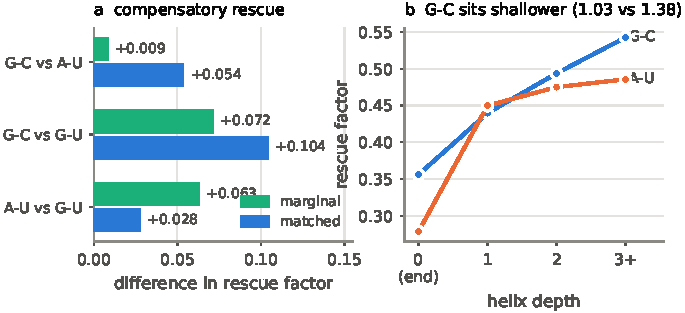
\includegraphics[width=0.86\linewidth]{fig5_rescue.pdf}
\caption{\textbf{Rescue by pair type, marginal and matched.} The readout is the fraction of the
wild-type profile a compensatory double mutant restores, so a higher value means the pair the
mutation was designed to test is more likely to have been really there. Matching is within
(design, helix depth, crossed); the marginal bars are the same pairs unstratified, and the gap
between the two panels is what \S\ref{sec:mediation} decomposes.}
\label{fig:rescue}
\end{figure}

\paragraph{Why this readout answers the question the design score cannot.} A design score is a
property of a whole molecule under a scoring rule, so a sequence property that raises it might be
raising the rule's opinion. Rescue is a property of one pair under an intervention on that pair. A
different structure that happens to explain the wild-type profile is not restored by this
particular double mutation, so structural degeneracy, which limits what a profile-matching score
can conclude, does not reach this statistic. \emph{One number belongs in Methods rather than here}:
the detection ladder for these two contrasts clears the observed effect by
$\jdg{rescueAUMargin}\times$ and $\jdg{rescueGUMargin}\times$, so this is a real but not a
comfortable margin, and the ladder returns $\jdg{rescueAUDelta0}$ at zero injected effect.

% =====================================================================
\section{Placement accounts for most of what the marginal contrast misses}
\label{sec:mediation}

The matched and marginal contrasts differ, and the mechanism is available in the same data. Two
quantities are computed \emph{without reference to each other}. The first is the effect of depth on
rescue: within (design, crossed), regressing rescue on depth gives $\beta_{\mathrm{depth}} =
\jdg{medBeta}$ per depth unit. The second is where the pair types sit: G--C pairs are
$\jdg{medGap}$ depth units shallower than A--U pairs, pooled over designs. Their product is what
placement predicts the marginal contrast should lose.

\begin{claimbox}
\textbf{The decomposition closes to $\jdg{medFrac}$.} Marginal $\jdg{medMarginal}$ against matched
$\jdg{medMatched}$ is an attenuation of $\jdg{medObs}$; $\beta_{\mathrm{depth}}$ times the depth
gap predicts $\jdg{medPred}$. \emph{Predicted and observed are separate calculations that meet},
which is what makes this a decomposition rather than the observation that two things correlate. The
remaining $\approx 29\%$ is not attributed here.
\end{claimbox}

\begin{figure}[!htbp]
\centering
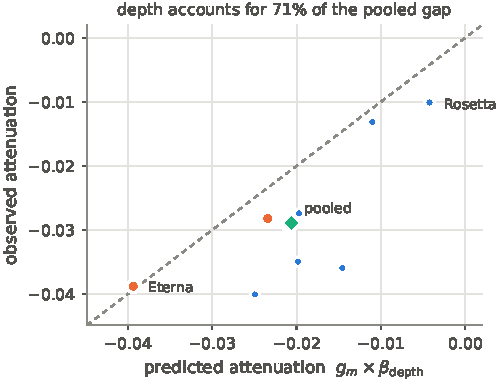
\includegraphics[width=0.52\linewidth]{fig6_mediation.pdf}
\caption{\textbf{Predicted against observed attenuation, one point per design method.} The
horizontal coordinate is that method's own depth gap times the pooled $\beta_{\mathrm{depth}}$, and
the vertical coordinate is its measured marginal-minus-matched difference; neither enters the
other's calculation. The diagonal is exact mediation. Every point sits below it, which is the
$\approx 29\%$ the decomposition does not claim, and the pooled diamond is the number in the text.
Orange marks the two human-designed arms.}
\label{fig:mediation}
\end{figure}

\paragraph{What this means for anyone measuring a sequence property on a designed corpus.} The
attenuation is not noise and it does not average away with more items, because it is produced by a
systematic design choice that is present in every design. A property correlated with position will
be measured at a fraction of its size, and the fraction is estimable exactly the way it is
estimated here: measure the covariate gap, measure the covariate's slope on the outcome, multiply.

% =====================================================================
\section{The same property on the benchmark's design score}
\label{sec:score}

The two sections above use an arm most benchmarks do not ship. This one asks what the property is
worth on the score every design in the corpus already has.

\textbf{Matched pairs of real molecules.} Within one target and one design method, we form all
ordered pairs of molecules whose global GC fraction differs by at most two percentage points and
whose shipped-panel prognostic score differs by at most $0.2$\,SD, and whose fraction of GC sitting
on target-paired positions differs by at least five percentage points. No model produces the
estimate; it is the pair-weighted mean difference of the benchmark's own score. \emph{The predictor
panel appears here for the first time in this paper, and only as a covariate}: no claim below
depends on any predictor being right.

\begin{table}[!htbp]
\centering\small
\caption{Matched-pair difference in OpenKnot points, six populations. Inference is by permutation
holding the matched design fixed (\S\ref{sec:methods}); the bootstrap interval is reported beside
it. Balance is the standardised mean difference on global GC. Two populations do not clear
$p \le 0.005$ and their $p$ is printed.}
\label{tab:score}
\begin{tabular}{@{}lrrrrr@{}}
\toprule
population & effect & $z$ & $p$ & pairs & SMD \\
\midrule
sample 2 (main) & $\jdg{cpop0Eff}$ & $\jdg{cpop0Z}$ & $\jdg{cpop0P}$ & $\jdg{cpop0N}$ & $\jdg{cpop0Smd}$ \\
baseline 4560   & $\jdg{cpop1Eff}$ & $\jdg{cpop1Z}$ & $\jdg{cpop1P}$ & $\jdg{cpop1N}$ & $\jdg{cpop1Smd}$ \\
sample 3        & $\jdg{cpop2Eff}$ & $\jdg{cpop2Z}$ & $\jdg{cpop2P}$ & $\jdg{cpop2N}$ & $\jdg{cpop2Smd}$ \\
batch 4         & $\jdg{cpop3Eff}$ & $\jdg{cpop3Z}$ & $\jdg{cpop3P}$ & $\jdg{cpop3N}$ & $\jdg{cpop3Smd}$ \\
batch 5 (blind) & $\jdg{cpop4Eff}$ & $\jdg{cpop4Z}$ & $\jdg{cpop4P}$ & $\jdg{cpop4N}$ & $\jdg{cpop4Smd}$ \\
batch 6 (blind) & $\jdg{cpop5Eff}$ & $\jdg{cpop5Z}$ & $\jdg{cpop5P}$ & $\jdg{cpop5N}$ & $\jdg{cpop5Smd}$ \\
\bottomrule
\end{tabular}
\end{table}

\begin{figure}[!htbp]
\centering
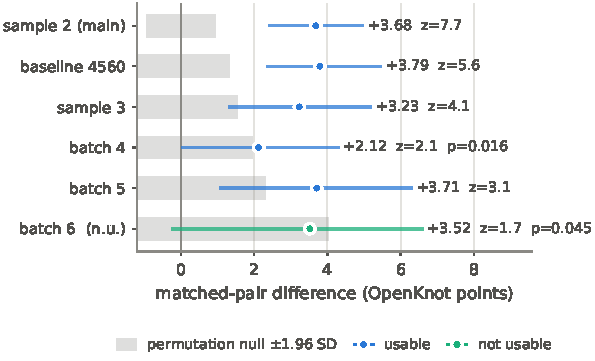
\includegraphics[width=0.70\linewidth]{fig3_matched.pdf}
\caption{\textbf{Matched-pair difference against the permutation null.} Effects are positive in
all six populations and $\jdg{cSigStrict}$ of $\jdg{c5N}$ clear $p \le 0.005$; balance on global GC
is at most $\jdg{cSmdHi}$ throughout.}
\label{fig:matched}
\end{figure}

\subsection{Three cuts against probing chemistry}
\label{sec:cuts}

The score rewards low reactivity at paired positions, and 2A3 reactivity depends on base identity,
so ``more GC at paired positions scores better'' has a chemistry explanation. Each cut below fails
under that explanation in a different way.

\textbf{Circular shift.} Rotating the target's paired-position set leaves the number of positions
and the run structure intact and destroys the alignment. Shifted arms return $\jdg{p4Lo}$ to
$\jdg{p4Hi}$ against a real effect of $\jdg{cEffLo}$ to $\jdg{cEffHi}$, passing on
$\jdg{p4Pass}$ of $\jdg{c5N}$ populations. The leak diagnostic confirms the placebo is not a weak
version of the treatment: shifted arms admit a true placement gap of $\jdg{p4LeakLo}$ to
$\jdg{p4LeakHi}$ against the real arm's $\jdg{p4RealLo}$ to $\jdg{p4RealHi}$, about
$\jdg{p4LeakPct}$.

\textbf{Pairing against composition, blind.} Holding the GC \emph{base-pair} fraction fixed and
varying placement beats holding placement fixed and varying composition, at every stringency: the
pairing arm clears $p \le 0.005$ on $\jdg{d2PLo}$ to $\jdg{d2PHi}$ of $\jdg{c5N}$ populations and
the composition arm on $\jdg{d2CLo}$ to $\jdg{d2CHi}$. The registered primary comparison is the
slope, which is $\jdg{d2SlopeP04}$ against $\jdg{d2SlopeC04}$ at the loosest stringency.

\textbf{A sign test on single-nucleotide interventions.} Breaking a target pair from either side
raises partner reactivity and lowers expected correctness, on all four arms:
$\jdg{d3Y0}$, $\jdg{d3Y1}$, $\jdg{d3Y2}$, $\jdg{d3Y3}$ upward and $\jdg{d3E0}$, $\jdg{d3E1}$,
$\jdg{d3E2}$, $\jdg{d3E3}$ downward, with $\jdg{d3NPos}$ and $\jdg{d3NNeg}$ of four intervals
excluding zero on the two readouts. \emph{Only the sign is used, and deliberately}: the partner
base's own identity differs across the four arms, so their magnitudes are not comparable, whereas
the chemistry hypothesis makes a prediction about direction --- breaking a G--C pair from the G
side should look \emph{better} --- and no arm reverses.

\textbf{Robustness to the corpus authors' own structure filter.} Restricting to designs the
benchmark's own predictor scores above $\jdg{c5Cut}$ leaves the effects essentially unchanged and
$\jdg{c5Sig}$ of $\jdg{c5N}$ populations clearing $p \le 0.005$.

\begin{figure}[!htbp]
\centering
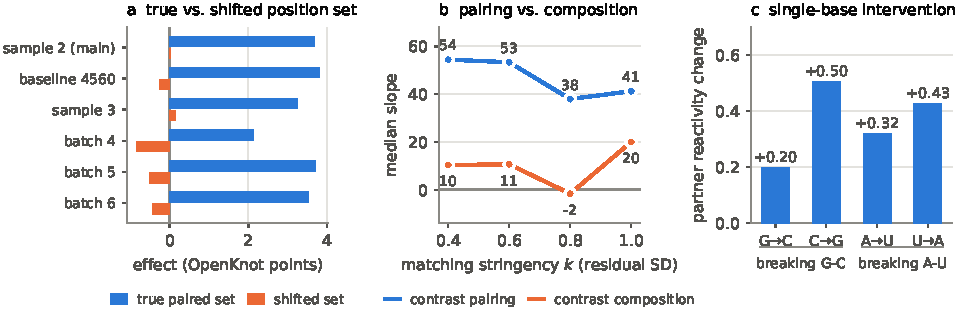
\includegraphics[width=0.92\linewidth]{fig4_three_cuts.pdf}
\caption{\textbf{The three cuts.} Left, real against circularly shifted placement. Centre, the
pairing arm against the composition arm at every stringency. Right, the four single-nucleotide
arms on both readouts, where only the sign carries the argument.}
\label{fig:cuts}
\end{figure}

% =====================================================================
\section{The placement gradient is a property of the design method}
\label{sec:gradient}

The confound of \S\ref{sec:mediation} is a design choice, so it should vary with who designed. Nine
methods produced designs for the same twenty targets, which makes the depth gap decomposable into a
target component and a method component. \emph{This arm never touches the outcome variable}: it is
computed from target structures and sequences alone.

\begin{figure}[!htbp]
\centering
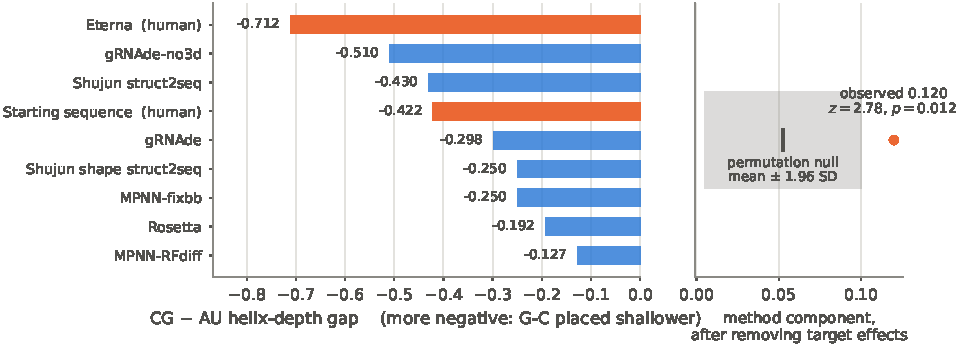
\includegraphics[width=0.94\linewidth]{fig7_gradient.pdf}
\caption{\textbf{Left: the G--C-minus-A--U depth gap, by design method.} Every method places G--C
shallower, and the spread across methods is $\jdg{gSpread}$ depth units, from $\jdg{gGapMin}$
(\texttt{\jdg{gGapMinName}}) to $\jdg{gGapMax}$ (\texttt{\jdg{gGapMaxName}}). \textbf{Right: the
method component after removing target main effects}, against the permutation null of method
labels within target. Nothing in this figure involves rescue.}
\label{fig:gradient}
\end{figure}

\begin{claimbox}
\textbf{Reported as suggestive, at three strengths.} The method component is $\jdg{gMethComp}$
against a null of $\jdg{gNullMean} \pm \jdg{gNullSd}$, $z = \jdg{gZ}$, $p = \jdg{gP}$ on
$\jdg{gCells}$ (method, target) cells; the human-designed arm is at rank $\jdg{gHumanRank}$ of
$\jdg{gNMethods}$ on the gradient, which was the registered prediction; and the cross-method slope
of observed attenuation on predicted is $\jdg{gSlope}$ with permutation $p = \jdg{gSlopeP}$ at
$n = \jdg{gSlopeN}$. \emph{None of the three clears a $0.005$ bar alone, and the reason is
legible on the instrument}: the observed spread of $\jdg{gSpread}$ sits between the ladder rungs
where detection is $\jdg{gLadLo}$ and $\jdg{gLadHi}$, so this arm is at its own detection edge for
the effect present. A larger design pool, not a different analysis, is what would settle it.
\end{claimbox}

\paragraph{The competing explanation, and why the decomposition is the test for it.} Placing G--C
at helix ends is also thermodynamics: a closing G--C avoids the terminal A--U penalty, so a method
that optimises or learns stability would arrive at the same preference without any heuristic. That
prediction is specific and it is the reason this arm is a decomposition: a thermodynamic preference
is a property of the \emph{target} and would leave the method component at the null, while a design
rule is a property of the \emph{method}. Both components are reported, and the target component is
much the larger of the two at $\jdg{gTgtComp}$.

% =====================================================================
\section{Methods that carry a claim}
\label{sec:methods}

\textbf{Permutation must hold the design fixed.} Where an estimator is a matched-pair difference
under calipers, and a caliper column is jointly structured with the treatment, permuting the
treatment \emph{rebuilds} the matched set rather than relabelling it, and the resulting null is
computed on a larger and easier design. Permuting the outcome within cell holds the matched set
fixed and is the same null in the limit, since shuffling molecule identity while carrying every
covariate is equivalent to shuffling the outcome. Measured type-I error at a nominal $0.005$:
$\jdg{nullRateOld}$ for the treatment-side permutation against $\jdg{nullRateNew}$ for the
outcome-side one. The equivalence was checked directly, with SD ratios of $\jdg{verSdLo}$ to
$\jdg{verSdHi}$ and a largest two-sample KS statistic of $\jdg{verKsHi}$ against a $5\%$ critical
value of $\jdg{verKsCrit}$.

\textbf{Ladders are built on zero.} Every detection ladder in this paper scrambles labels first, so
the true effect is zero, then injects a known effect. A ladder whose zero rung does not fall back
to nominal is void and is not used.

\textbf{Preregistration.} Every criterion graded here was frozen in a declaration file committed
and pushed before the corresponding runner existed, and verdicts are reported in the declaration's
own wording, including where a staked prediction failed.

% =====================================================================
\section{Limitations}
\label{sec:limits}

\textbf{(i) One corpus.} All measurements are on a single chemical-probing benchmark. Every
mechanism is stated so that it is checkable elsewhere, and none has been checked elsewhere by us.

\textbf{(ii) Observational.} We did not choose which sequences exist. \S\ref{sec:rescue} and
\S\ref{sec:cuts} are interventional at the level of the \emph{mutation}, which is what licenses the
formation claim; the placement claim is not, and \S\ref{sec:gradient}'s method comparison is not a
randomised assignment of methods.

\textbf{(iii) No sequence was synthesised.} Nothing here was tested by building a molecule to the
rule and measuring it. That is the one experiment that would convert \S\ref{sec:score} from a
selection result into a construction result, and it needs a tube.

\textbf{(iv) The compensatory arm covers good designs only.} It measured the best-scoring design
per (target, method), so the pair-level results are conservative with respect to poor designs and
do not extrapolate to them.

\textbf{(v) Prior art on the placement rule.} GC placement as a design heuristic predates this
work. What is measured here is its effect on pair formation and on the measurement itself.

% =====================================================================
\section{Conclusion}
\label{sec:conclusion}

Whether a designed base pair forms depends on what the pair is, and the dependence is measurable
with an intervention rather than inferred from a predictor: matched on placement, a G--C target
pair is recovered $\jdg{rescueAU}$ more than an A--U pair and $\jdg{rescueGU}$ more than a G--U
pair. How much of that a study sees depends on something the study did not choose, because the
designers who built the corpus already put G--C shallower, and that placement accounts for
$\jdg{medFrac}$ of the difference between the marginal and matched contrasts. On the benchmark's
own design score the same property is worth $\jdg{cEffLo}$ to $\jdg{cEffHi}$ points between two
real molecules matched on everything else we could match.

The portable part is the second finding rather than the first. A corpus of designed molecules
carries its designers' rules as covariates, and any sequence property correlated with position will
be measured at a fraction of its true size on such a corpus. That fraction is estimable from the
corpus itself, by measuring the covariate gap and the covariate's slope and multiplying, and here
it recovers $\jdg{medFrac}$ of the discrepancy it was asked to explain.

% =====================================================================
\bibliographystyle{plainnat}
\bibliography{refs}

\end{document}
